\chapter{Sistema de informação: análise de requisitos e arquitetura}





\section{Análise de requisitos}



\section{Diagramas}


\subsection{Entidade-relação}


\subsection{Modelo relacional}


\subsection{Estrutura final}



\section{Requisitos de funcionamento}



\section{Tecnologias de desenvolvimento}





\subsection{\textit{Web}}


\subsection{Base de dados}


\subsection{\textit{Mobile}}





\section{title}
\newpage 

\section{Casos de utilização}

\begin{figure}[!htb]
	\centering
	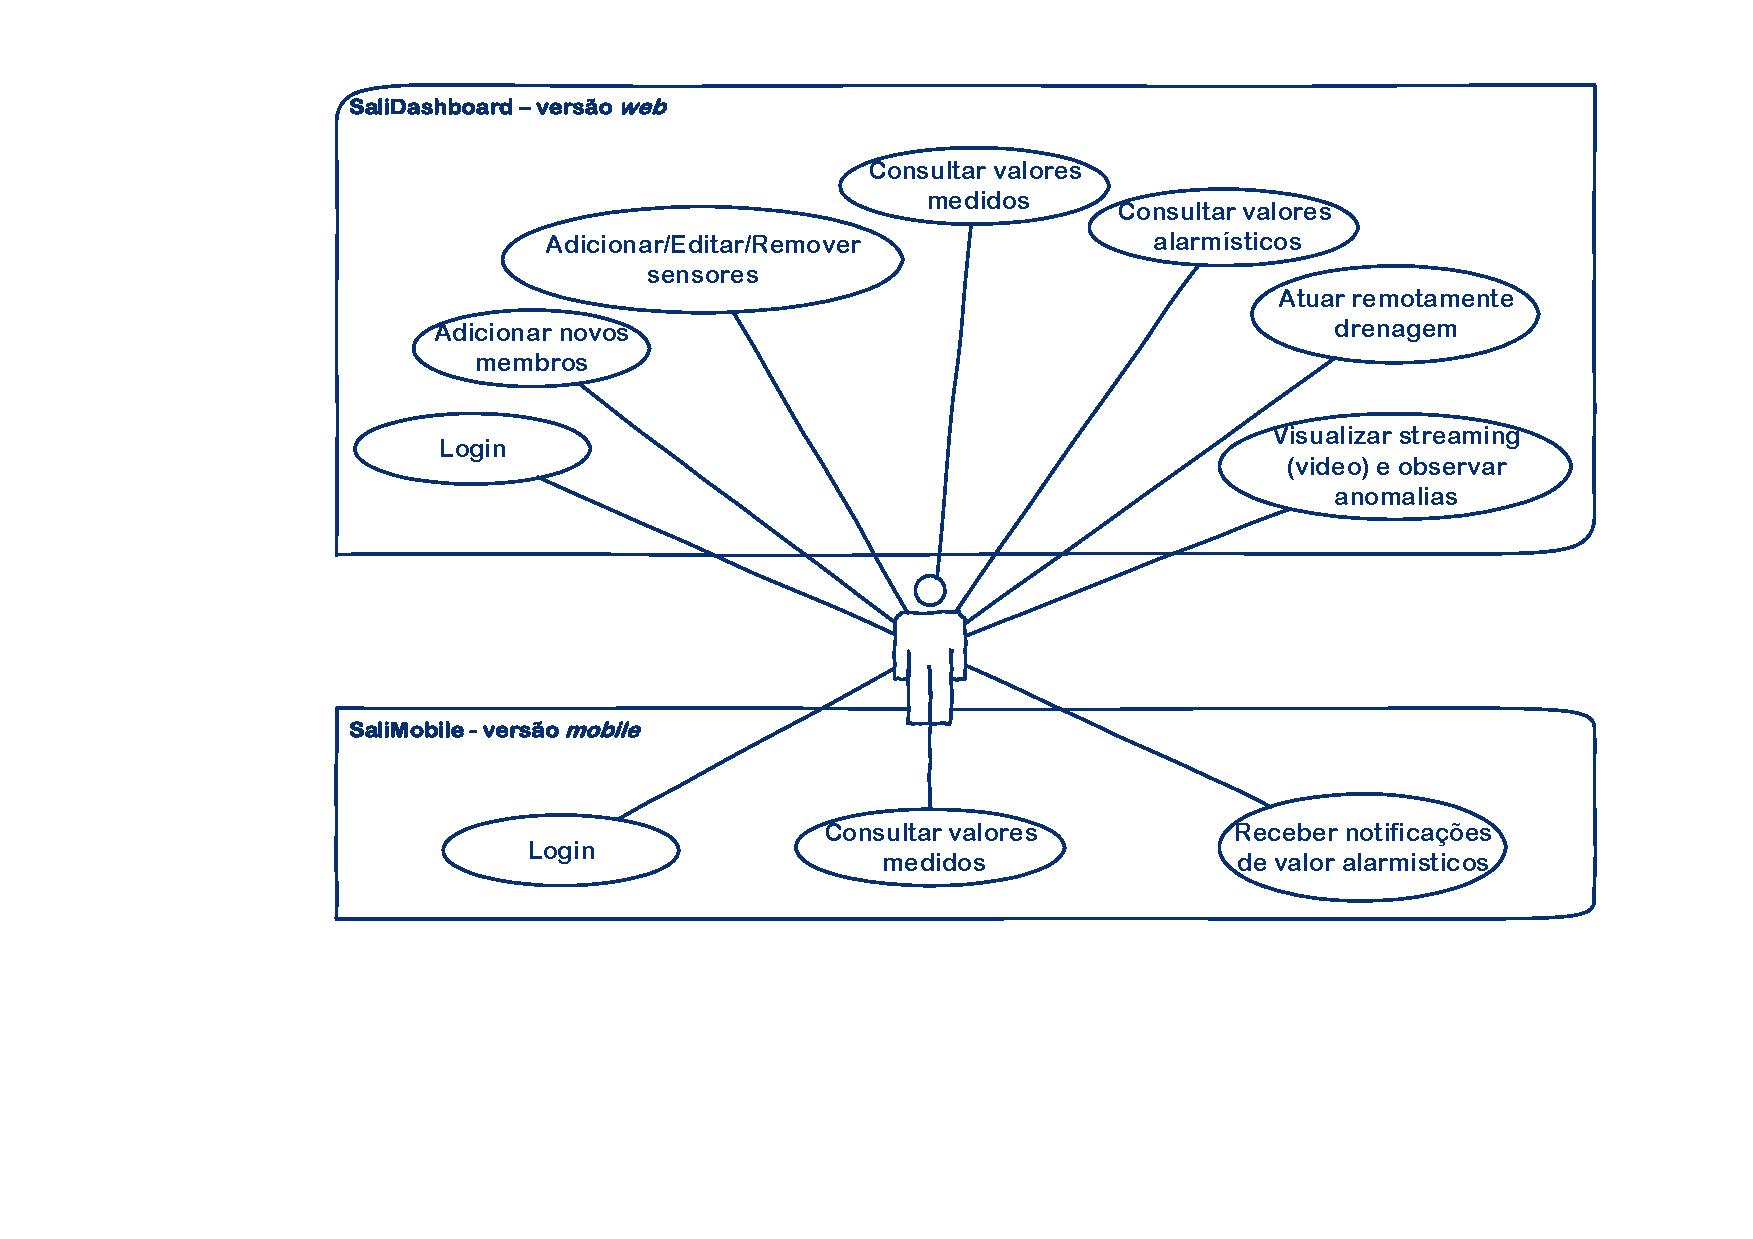
\includegraphics[scale=0.5]{esquemas/usecases.pdf}
	\caption{Pirâmide do conhecimento: modelo DIKW}
	\label{dikw}
\end{figure}








\section{API rest}



app mobile
microcontroladores -> controller modulers 


documentação com swager 



\section{\textit{Deploy} do projecto}

https://jee-appy.blogspot.com.tr/2015/04/deploy-django-project-on-apache-using.html

Caracteristicas da maquina virtual

Description:	Ubuntu 14.04.1 LTS
64 bits
RAM 2GB 



